% depgraph-item.tex -- a minimal item-dependency-graph example.

\documentclass[tikz,border=3pt]{standalone}

\usepackage[dvipsnames]{xcolor}
\usetikzlibrary{arrows.meta,calc,positioning}

\newcommand{\WR}{\mathsf{WR}}
\newcommand{\WW}{\mathsf{WW}}
\newcommand{\RW}{\mathsf{RW}}

\begin{document}
  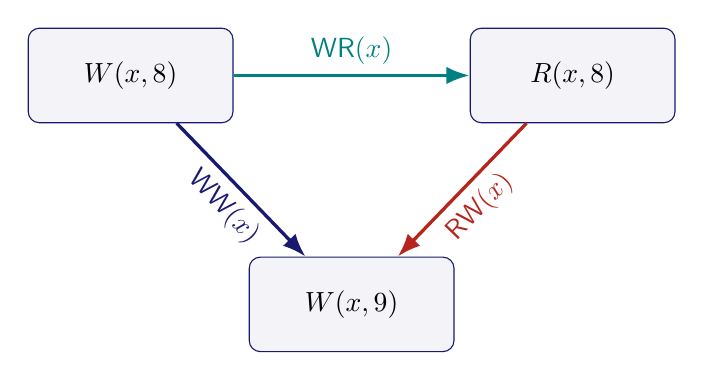
\begin{tikzpicture}[
    >=Latex,
    font=\sffamily,
    op/.style={
      draw=MidnightBlue,
      rounded corners=4pt,
      fill=MidnightBlue!5,
      minimum width=26mm,
      minimum height=12mm,
      align=center,
    },
  ]
    \node[op] (w2) {\textbf{$W(x,8)$}};
    \node[op,right=30mm of w2] (r2) {\textbf{$R(x,8)$}};
    \node[op,below=23mm of $(w2)!0.5!(r2)$] (w3) {\textbf{$W(x,9)$}};

    \draw[-Latex,very thick,teal]
      (w2) -- node[above, font=\normalsize] {$\WR(x)$} (r2);
    \draw[-Latex,very thick,MidnightBlue]
      (w2) -- node[below, font=\normalsize, sloped] {$\WW(x)$} (w3);
    \draw[-Latex,very thick,BrickRed]
      (r2) -- node[below, font=\normalsize, sloped] {$\RW(x)$} (w3);
  \end{tikzpicture}
\end{document}